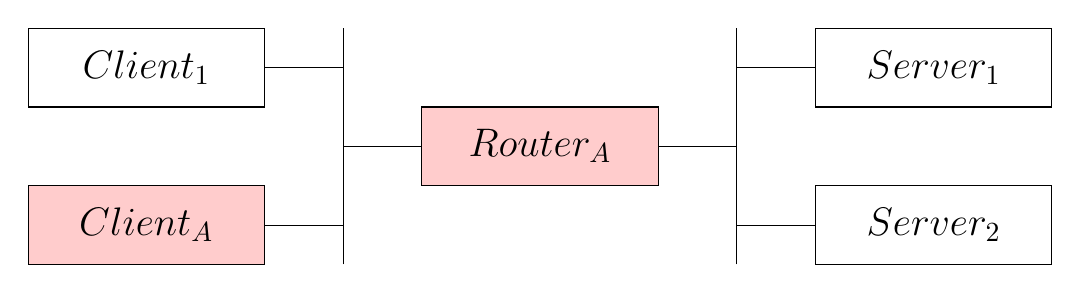
\begin{tikzpicture}[font=\Large,
    arrow/.style={thick,<->,shorten >=2pt,shorten <=2pt,>=stealth},
]
    \draw[fill=red!20!white] (0,0) rectangle (3,1) node [pos=.5] {$Client_{A}$};
    \draw (0,2) rectangle (3,3) node [pos=.5] {$Client_1$};
    
    \draw[fill=red!20!white] (5,1) rectangle (8,2) node [pos=.5] {$Router_{A}$};

    \draw (10,0) rectangle (13,1) node [pos=.5] {$Server_{2}$};
    \draw (10,2) rectangle (13,3) node [pos=.5] {$Server_{1}$};
    
    \draw (3,.5) -- (4,.5); 
    \draw (3,2.5) -- (4,2.5); 
    \draw (4,1.5) -- (5,1.5);
    \draw (4,0) -- (4,3);

    \draw (9,.5) -- (10,.5); 
    \draw (9,2.5) -- (10,2.5); 
    \draw (8,1.5) -- (9,1.5);
    \draw (9,0) -- (9,3);
\end{tikzpicture}
